% Based on: diffusion-for-failures paper (DEFT).

\chapter{Diffusion Under Failure-Induced Embodiments}
\label{ch:failures}

\section{Revisiting the Long-Deployment Failure Problem}
\label{sec:failures:revisit}

The Mars rover Opportunity's robotic arm first stalled on November 25, 2005; its shoulder joint experienced intermittent motor stalls for years, managed with voltage workarounds and revised stow procedures. Similarly, Curiosity's drill paused sampling for roughly eighteen months until a hand-designed drilling method restored coring \cite{nasa_science_first_drilled_sample_2018,jpl_opportunity_shoulder_2008}. Cases like these underscore that failures in continuously operating systems are inevitable \cite{factory_efficiency_2020}. Prevailing safety standards mandate \textsl{fail-freeze} behavior, requiring robots to halt when faults are detected \cite{ISO10218-1,ISO13849-1,IEC60204-1}. The result is prolonged downtime and reduced autonomy.
In this work, we contrast this overly conservative approach with \textsl{fail-active} behavior, a more ambitious (and harder to achieve) reliability goal in which robots maintain functionality, full or reduced, under fault conditions \cite{aero_reliability}. \textbf{Fail-active behavior is how humans operate}: we continue walking on a sprained ankle, writing with a non-dominant hand, going to work when we've had our hearts broken.

Faults reshape what the robot can physically do: actuation failures (e.g., joint range and velocity restrictions) shrink the feasible workspace and degrade manipulability, electrical faults (e.g., brownouts) reduce control authority, sensor drift can distort state estimates, and end-effector wear (e.g. lowered friction) degrades contact mechanics. Ultimately, these physical changes mean the robot can no longer move the way it originally planned.

In this chapter, we focus on \textit{actuation failures} as they directly affect how the robot moves. \textit{Fail-active} operation requires adapting to these altered kinematics, which can cause end-effector motion to become non-holonomic; meaning the same control input may no longer yield the same end-effector motion \cite{Bloch_Krishnaprasad_Murray_2016}.
It is also important to note that since degradation can evolve over time \cite{barbieri2015sensor} and the failure state is not known a priori, \textbf{the space of failure modes is effectively unbounded}. Moreover, each joint can fail independently in multiple ways, and this complexity scales combinatorially with the robot's degrees of freedom, \textbf{making reliable performance across failures hard to engineer}.

As failure-induced constraints redefine the robot's workspace, manipulability, and feasible interactions with the world, \textsl{we posit that each failure mode can be interpreted as a new embodiment}.
Through this lens, different embodiments are unable to perform the same tasks using the same behaviors. As no same set of behaviors can span all embodiments, multiple motion primitives are needed to expand the feasible action space and reachable task-space \cite{briscoe2024exploring}.

Synthesizing effective motion primitives for arbitrary failure conditions is challenging due to the complex relationship between robot embodiment constraints and feasible task-space behaviors. Existing approaches fall short in three key gaps: 1) they do not generalize to arbitrary failure configurations \cite{briscoe2024exploring,xie2021maximizing}; 2) they are not capable of completing multiple manipulation primitives \cite{pham2024adaptive}; and 3) they do not address multi-joint failures \cite{mu2016kinematic,kim2024quadrupedal}. To the best of the authors' knowledge, no existing work bridges all three of these gaps simultaneously.
Diffusion models are uniquely suited to solve this. Because they excel at modeling multimodal data distributions, diffusion policies can generate across the range of actions required to span these infinite embodiments at inference.

\begin{figure}
    \centering
    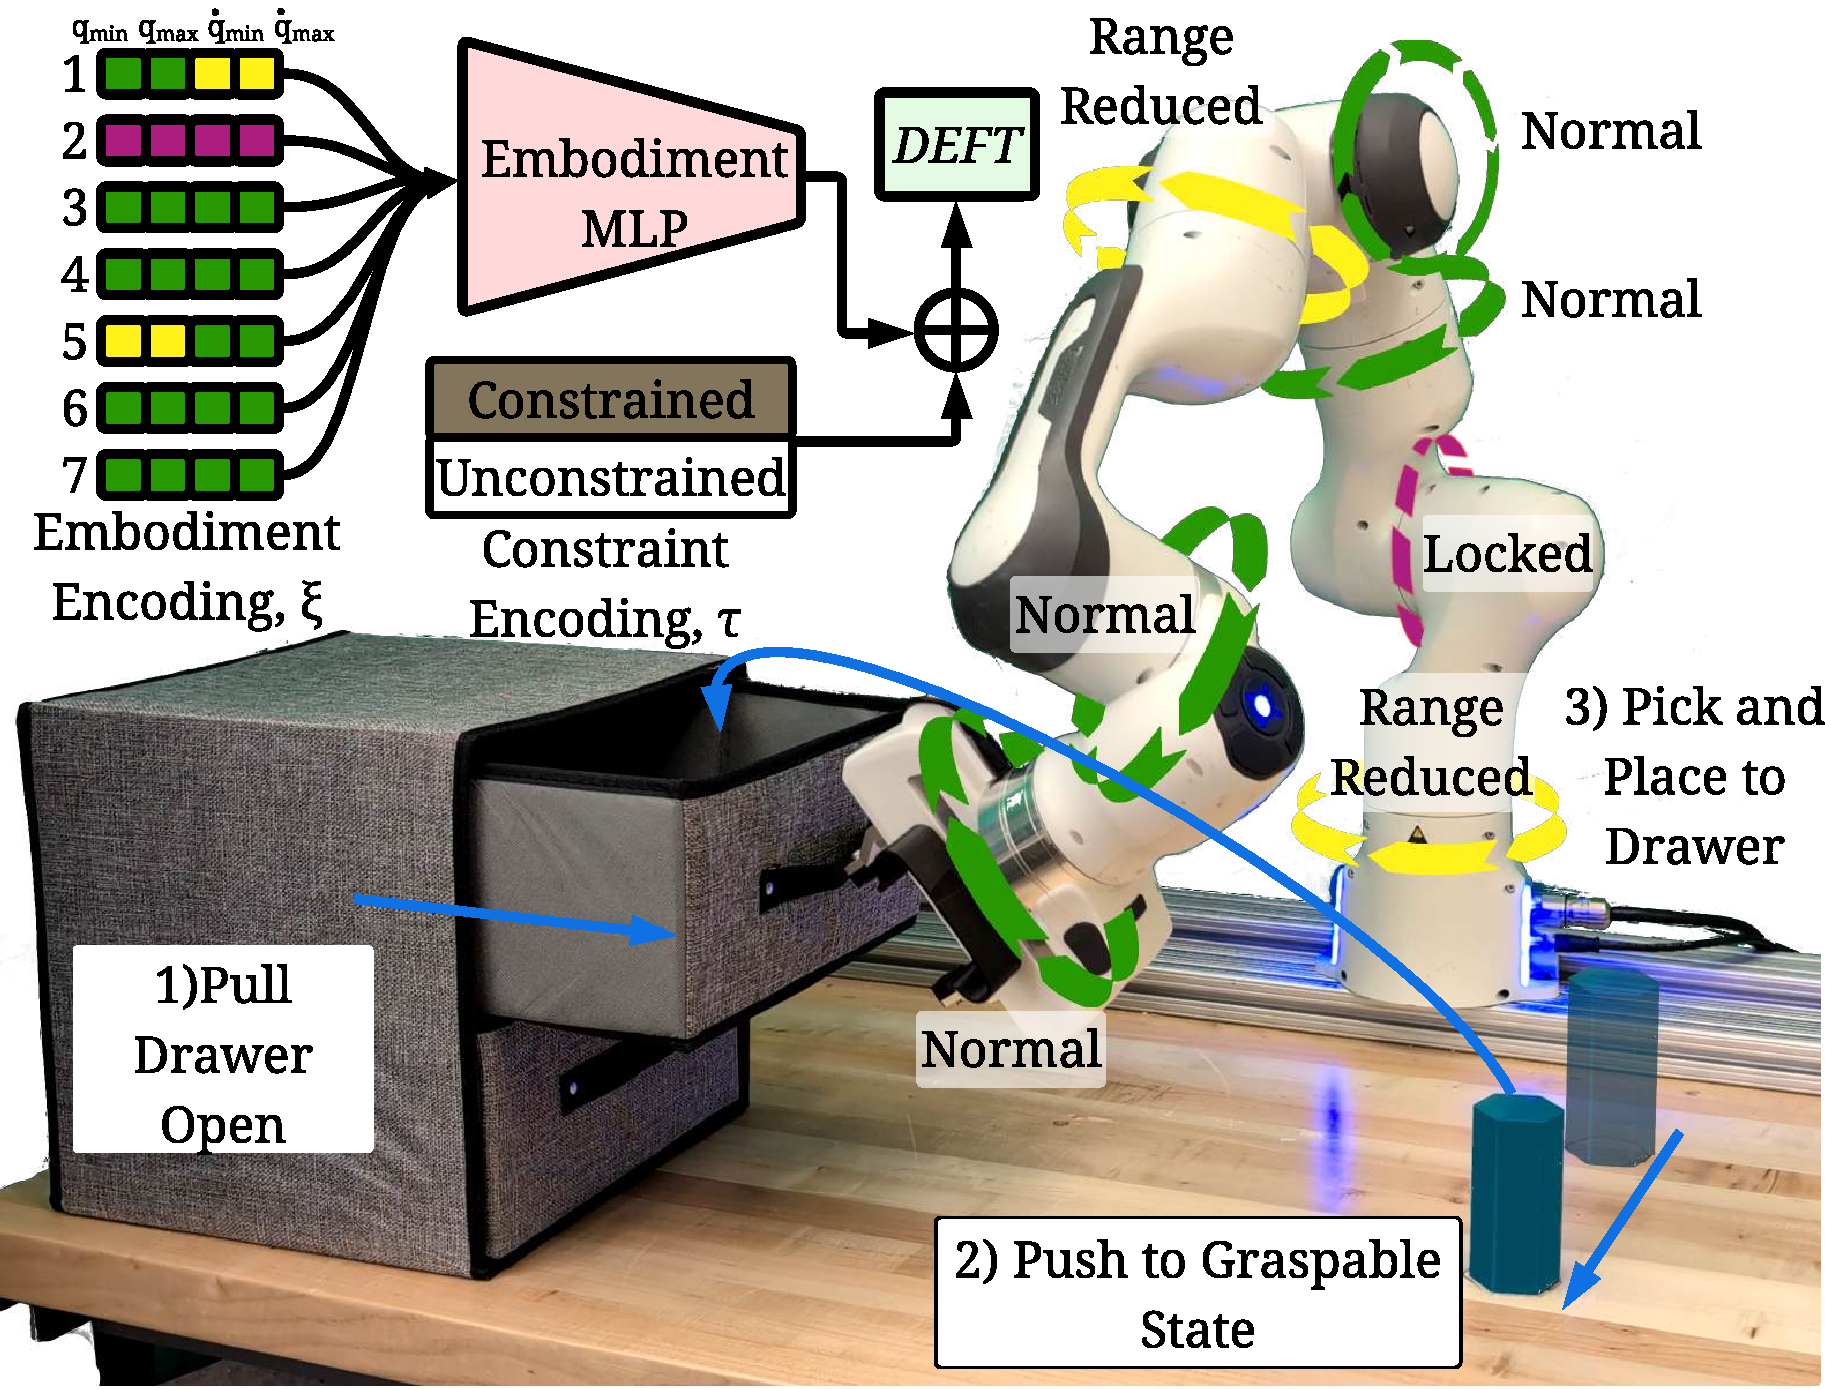
\includegraphics[width=\columnwidth]{../movingon/figures/first_page_figure_compressed.pdf}
    \caption{DEFT takes as input a structured embodiment encoding representing joint-level failures and a constraint encoding then synthesizes a feasible robot trajectory via a diffusion model. After experiencing a failure, a given task will likely need to be completed in a different manner. In this figure, the pick-and-place segment is no longer feasible, given the failure condition of a locked second joint and reduced velocity range on joint 1 and reduced angle range on joint 5, and the robot must now push the object to a graspable state to complete the task.}
    \label{fig:deft:first}
\end{figure}

\section{Conditioning on High-Level Encodings of Task Constraints}
\label{sec:failures:conditioning}

To this end, we present \textit{DEFT}: a \textit{D}iffusion-based \textit{E}mbodiment-aware \textit{F}ail-active \textit{T}ask-conditioned trajectory generation framework, capable of maintaining robot manipulation functionality under failure conditions (\cref{fig:deft:first}). Our contributions are:
(i) an \textit{embodiment vector} encoding per-joint actuation failures for online adaptation to previously unseen failure-induced embodiments and
(ii) a \textit{constraint encoding} selecting between constrained and unconstrained motions to enable the use of multiple motion primitives.
Furthermore, we utilize start--goal inpainting and output clamping to enforce embodiment failure conditions \cite{repaint_lugmayr_2022}.

\begin{figure*}
  \centering
  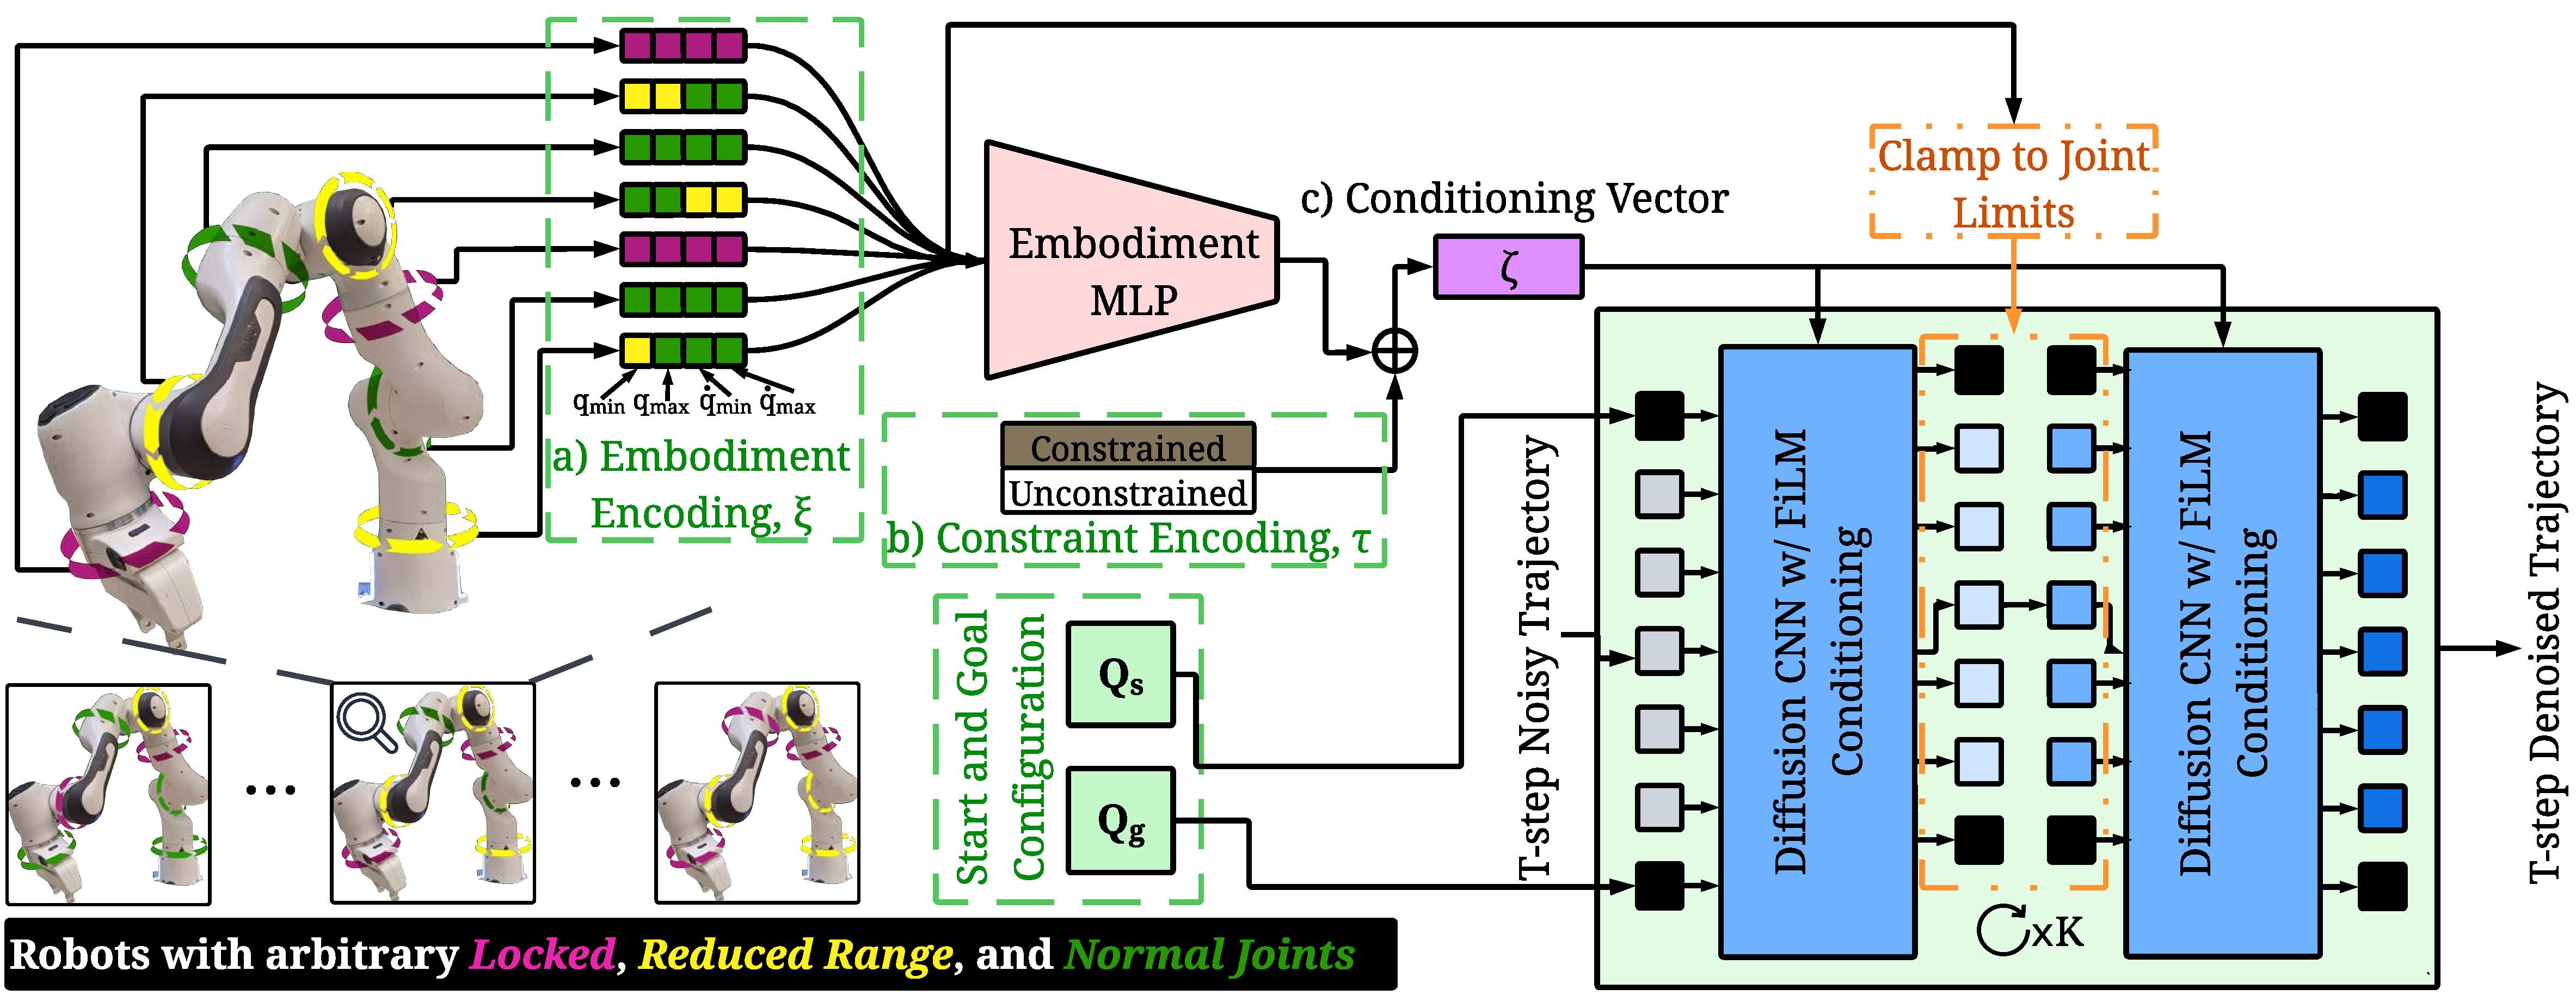
\includegraphics[width=\textwidth]{../movingon/figures/block_diagram.pdf}
  \caption{Overview of DEFT. (a) joint-level embodiment constraints are encoded into a structured representation capturing failure constrained joint position and velocity limits. This embodiment encoding is processed by a multilayer perceptron (MLP) and used to condition the diffusion model. (b) Task-specific constraints (e.g.\ unconstrained or constrained) are represented as one-hot vectors and concatenated with the embodiment encoding to constrain the generative process.
  Given these conditioning signals and start--goal joint configurations, the model generates feasible joint-space trajectories adapted explicitly to both the robot's degraded embodiment and task requirements. At each step of the denoising process the predicted joint values are clamped to the failure-induced robot joint limits.}
  \label{fig:deft:system}
\end{figure*}

Our goal is fail-active manipulation: generate functional, feasible trajectories under joint-level failures. We pose this as conditional trajectory generation given the failure-induced embodiment and the task constraint. Each failure specifies a new embodiment of the robot, and each constraint (e.g., \texttt{unconstrained} vs.\ \texttt{constrained} motion) induces a distinct trajectory distribution. Given the start and goal joint configurations the policy $\pi$ infers a future sequence of joint states over a fixed number of steps $T$. Unlike prior work that assumes a fixed set of failure configurations to control over, our method adapts online. It learns both the control behavior and the allowable motions from the current failure condition and the task constraint.

\paragraph{Embodiment Conditioning}
To inform the model of the robot's failure constrained embodiment, we use an embodiment encoding vector $\xi$ to condition the diffusion model. We model joint-level failures as per-joint constraints on the robot's actuation capabilities. Each failure embodiment is represented as $\xi = [\mathbf{e}_q, \mathbf{e}_{\dot{q}}] \in \mathbb{R}^{4N}$, with $\mathbf{e}_{q,j} = [q_j^{\min}, q_j^{\max}]^\top$ and $\mathbf{e}_{\dot{q},j} = [\dot{q}_j^{\min}, \dot{q}_j^{\max}]^\top$ for all $j \in \{1,\dots,N\}$ such that $\mathbf{0} \in \mathbf{e}_{\dot{q},j}$.
Failures reshape the robot's feasible configuration space and task-space reachability and exist in a continuous space, allowing $\xi$ to capture a wide spectrum of degradation severities, as shown in \cref{fig:deft:system}. Let $\{\mathbf{q}_t\}_{t=1}^T$ denote a trajectory over $T$ steps, where $\mathbf{q}_t \in \mathbb{R}^N$ is the joint configuration at time $t$, and $\dot{\mathbf{q}}_t$ its velocity. A configuration $\mathbf{q}_t$ satisfies the feasibility set $\mathcal{C}_t(\mathbf{q}_t,\xi)$ if:
\begin{equation}
\begin{aligned}
  \mathcal{C}_t(\mathbf{q}_t,\xi)=\Big\{\mathbf{q}_t\in\mathbb{R}^N\ \Big|\
  q_{t,j}\in \mathbf{e}_{q,j},\ \dot{q}_{t,j}\in \mathbf{e}_{\dot{q},j}\ \\ \ \forall j\in\{1,\dots,N\}\Big\}.
\end{aligned}
\end{equation}
A trajectory is feasible if $\mathbf{q}_{1:T}\in\bigcap_{t=1}^T \mathcal{C}_t(\mathbf{q}_t,\xi)$. We condition on failures structurally: the model learns to generate motion plans that obey the constraints.
To integrate embodiment information into the generative process, we pass $\xi$ through an MLP to produce an embedding that modulates the diffusion model via FiLM. To ensure that the trajectory connects the desired start and goal states we apply start--goal inpainting, fixing $(\mathbf{q}_s,\mathbf{q}_g)$ in the input trajectory. In addition, we clamp the trajectory to the limits during both training and inference.

\paragraph{Constraint Conditioning}
We further condition the model on discrete task constraints using a one-hot encoding vector, $\tau$. Let $\tau \in \{0,1\}^K$ be a one-hot vector with exactly one nonzero entry, such that
\[
\sum_{k=1}^{K} \tau_k = 1
\quad \text{and} \quad
\tau_k \in \{0,1\} \ \forall k.
\]
We concatenate $\tau$ with $\xi$ to form the conditioning vector $\zeta = [\xi, \tau]^\top$, which is injected via FiLM.
These constraints are not explicitly enforced during inference but must be learned implicitly through the conditioning signal. The constraint encoding also informs the model of task-imposed end effector constraints, which it otherwise would not know while operating in joint space.

\section{A Single Model Spanning Prehensile and Non-Prehensile Primitives}
\label{sec:failures:unified}

The formulation above enables zero-shot trajectory generation across diverse embodiments and task conditions. For example, when a shoulder joint becomes unusable, the robot can switch from lifting to pushing an object without task-specific retraining or policy switching.

We evaluate DEFT using two task constraints. \textit{Unconstrained} motion corresponds to a feasible trajectory between two points and includes unconstrained manipulation where the object is rigidly secured to the end-effector. \textit{Constrained} motion corresponds to planar, approximately straight-line motion with minimal end-effector orientation change---a spatial constraint for motion primitives such as pushing, pulling, or surface tracing. The valid trajectory sets are, respectively:
\begin{equation}
\begin{aligned}
  \mathcal{T}_\text{Unconstrained}=\Big\{\mathbf{q}_t \forall t\in\{1,\dots,T\}\ \Big|\
  & \mathbf{q}_1=\mathbf{q}_\text{s},\  \mathbf{q}_T=\mathbf{q}_\text{g},\ \\
  & \mathbf{q}_t\in \mathcal{C}_t(\mathbf{q},\xi)\Big\}.
\end{aligned}
\end{equation}
\begin{equation}
\begin{aligned}
  \mathcal{T}_\text{Constrained}
  = \Big\{\mathbf{q}_{t}\ \forall t\in\{1,\dots,T\}\ \Big|\ &
  \mathbf{p}_t\in\mathcal{P}\ \land\ \\ \Delta p_t\le \epsilon_p,
   \Delta \mathrm{R}_t\le \epsilon_R\ & \land\ \mathbf{q}_t\in \mathcal{C}_t(\mathbf{q},\xi)
  \Big\}.
\end{aligned}
\end{equation}

This allows \textsc{DEFT} to: 1) generalize to arbitrary failure configurations; 2) complete multiple manipulation primitives; and 3) handle multi-joint failures.

\section{Comparison with the Sampling-Based Approach}
\label{sec:failures:comparison}

We evaluate DEFT in two settings: (i) a \emph{simulation analysis} and (ii) a \emph{real-world comparison}. We ask if a single policy can remain \emph{fail-active} under embodiment degradation.

\paragraph{Simulation Analysis}
We test three hypotheses to probe DEFT's generalization to arbitrary joint failures (\textbf{H1} and \textbf{H2}) and to test whether DEFT produces both unconstrained and constrained motions (\textbf{H3}):
\begin{enumerate}
\item[\textbf{H.1}] Does DEFT obey embodiment constraints of arbitrary actuation failures more often than classical planners?
\item[\textbf{H.2}] Does DEFT \emph{generalize} to out-of-distribution (OOD) failures?
\item[\textbf{H.3}] Does DEFT adhere to constraint conditions more than approaches specialized to a single class of constraints?
\end{enumerate}

We use the motion planning method from data generation as our baseline, with RRT for \texttt{unconstrained} motions and differential IK with optimization for \texttt{constrained} motions. These baselines do not handle both primitives. In contrast, \textsc{DEFT} generates both within a unified model.

We evaluate on a fixed-base 7-DoF Franka Emika Panda arm. The study covers 4.7k failure conditions; of which 2.9k includes joint angle constraints (reduced and locked) and the rest are joint velocity constraints. For each condition, we randomly select 1--7 joints to be locked, range-limited, or velocity-restricted. Of these conditions, 22\% are in-domain (ID) and 78\% are out-of-domain (OOD). Each unique failure condition is tested 100 times, each with 100 start-goal pairs for a total of 4.7M trajectories evaluated.

\begin{table}[h]
\centering
\begin{tabular}{|c|c|c|c|}
\hline
\textbf{Hypothesis Summary} & \textbf{Test Condition}  & \textbf{Baseline} & \textbf{DEFT} \\ \hline
\textbf{H.1} Does DEFT handle & Angle Failure & 48.2\% & \textbf{84.3}\% \\ \cline{2-4}
arbitrary joint failures?& Velocity Failure & 32.5\% & \textbf{70.8}\% \\ \hline
\textbf{H.2} How well does DEFT & In Domain & \cellcolor{black} & \textbf{78.33\%} \\ \cline{2-4}
 handle unseen failures?& Out of Domain & \cellcolor{black} & \textbf{73.61\%} \\ \hline
\textbf{H.3} How well does DEFT  & Constrained & 30.93\% & \textbf{46.42}\% \\ \cline{2-4}
create multiple primitives?  & Unconstrained & 42.4\% & \textbf{99.58\%} \\ \hline
\end{tabular}
\caption{Success rate of the Baseline methods and the DEFT method.}
\label{tab:deft:performance}
\end{table}

\textsc{DEFT} consistently outperforms traditional planning baselines across various failure conditions (\cref{tab:deft:performance}). DEFT achieves a success rate of 74.51\% overall, while the baseline achieves only 36.85\%---an absolute improvement of 37.66 percentage points. Near-parity between ID and OOD success indicates DEFT extrapolates over joint space rather than memorizing seen cases. DEFT performs better for both primitives: 99.58\% vs.\ 42.40\% for unconstrained, and 46.42\% vs.\ 30.93\% for constrained motions.

\paragraph{Real-World Evaluation}

\begin{figure}
  \centering
  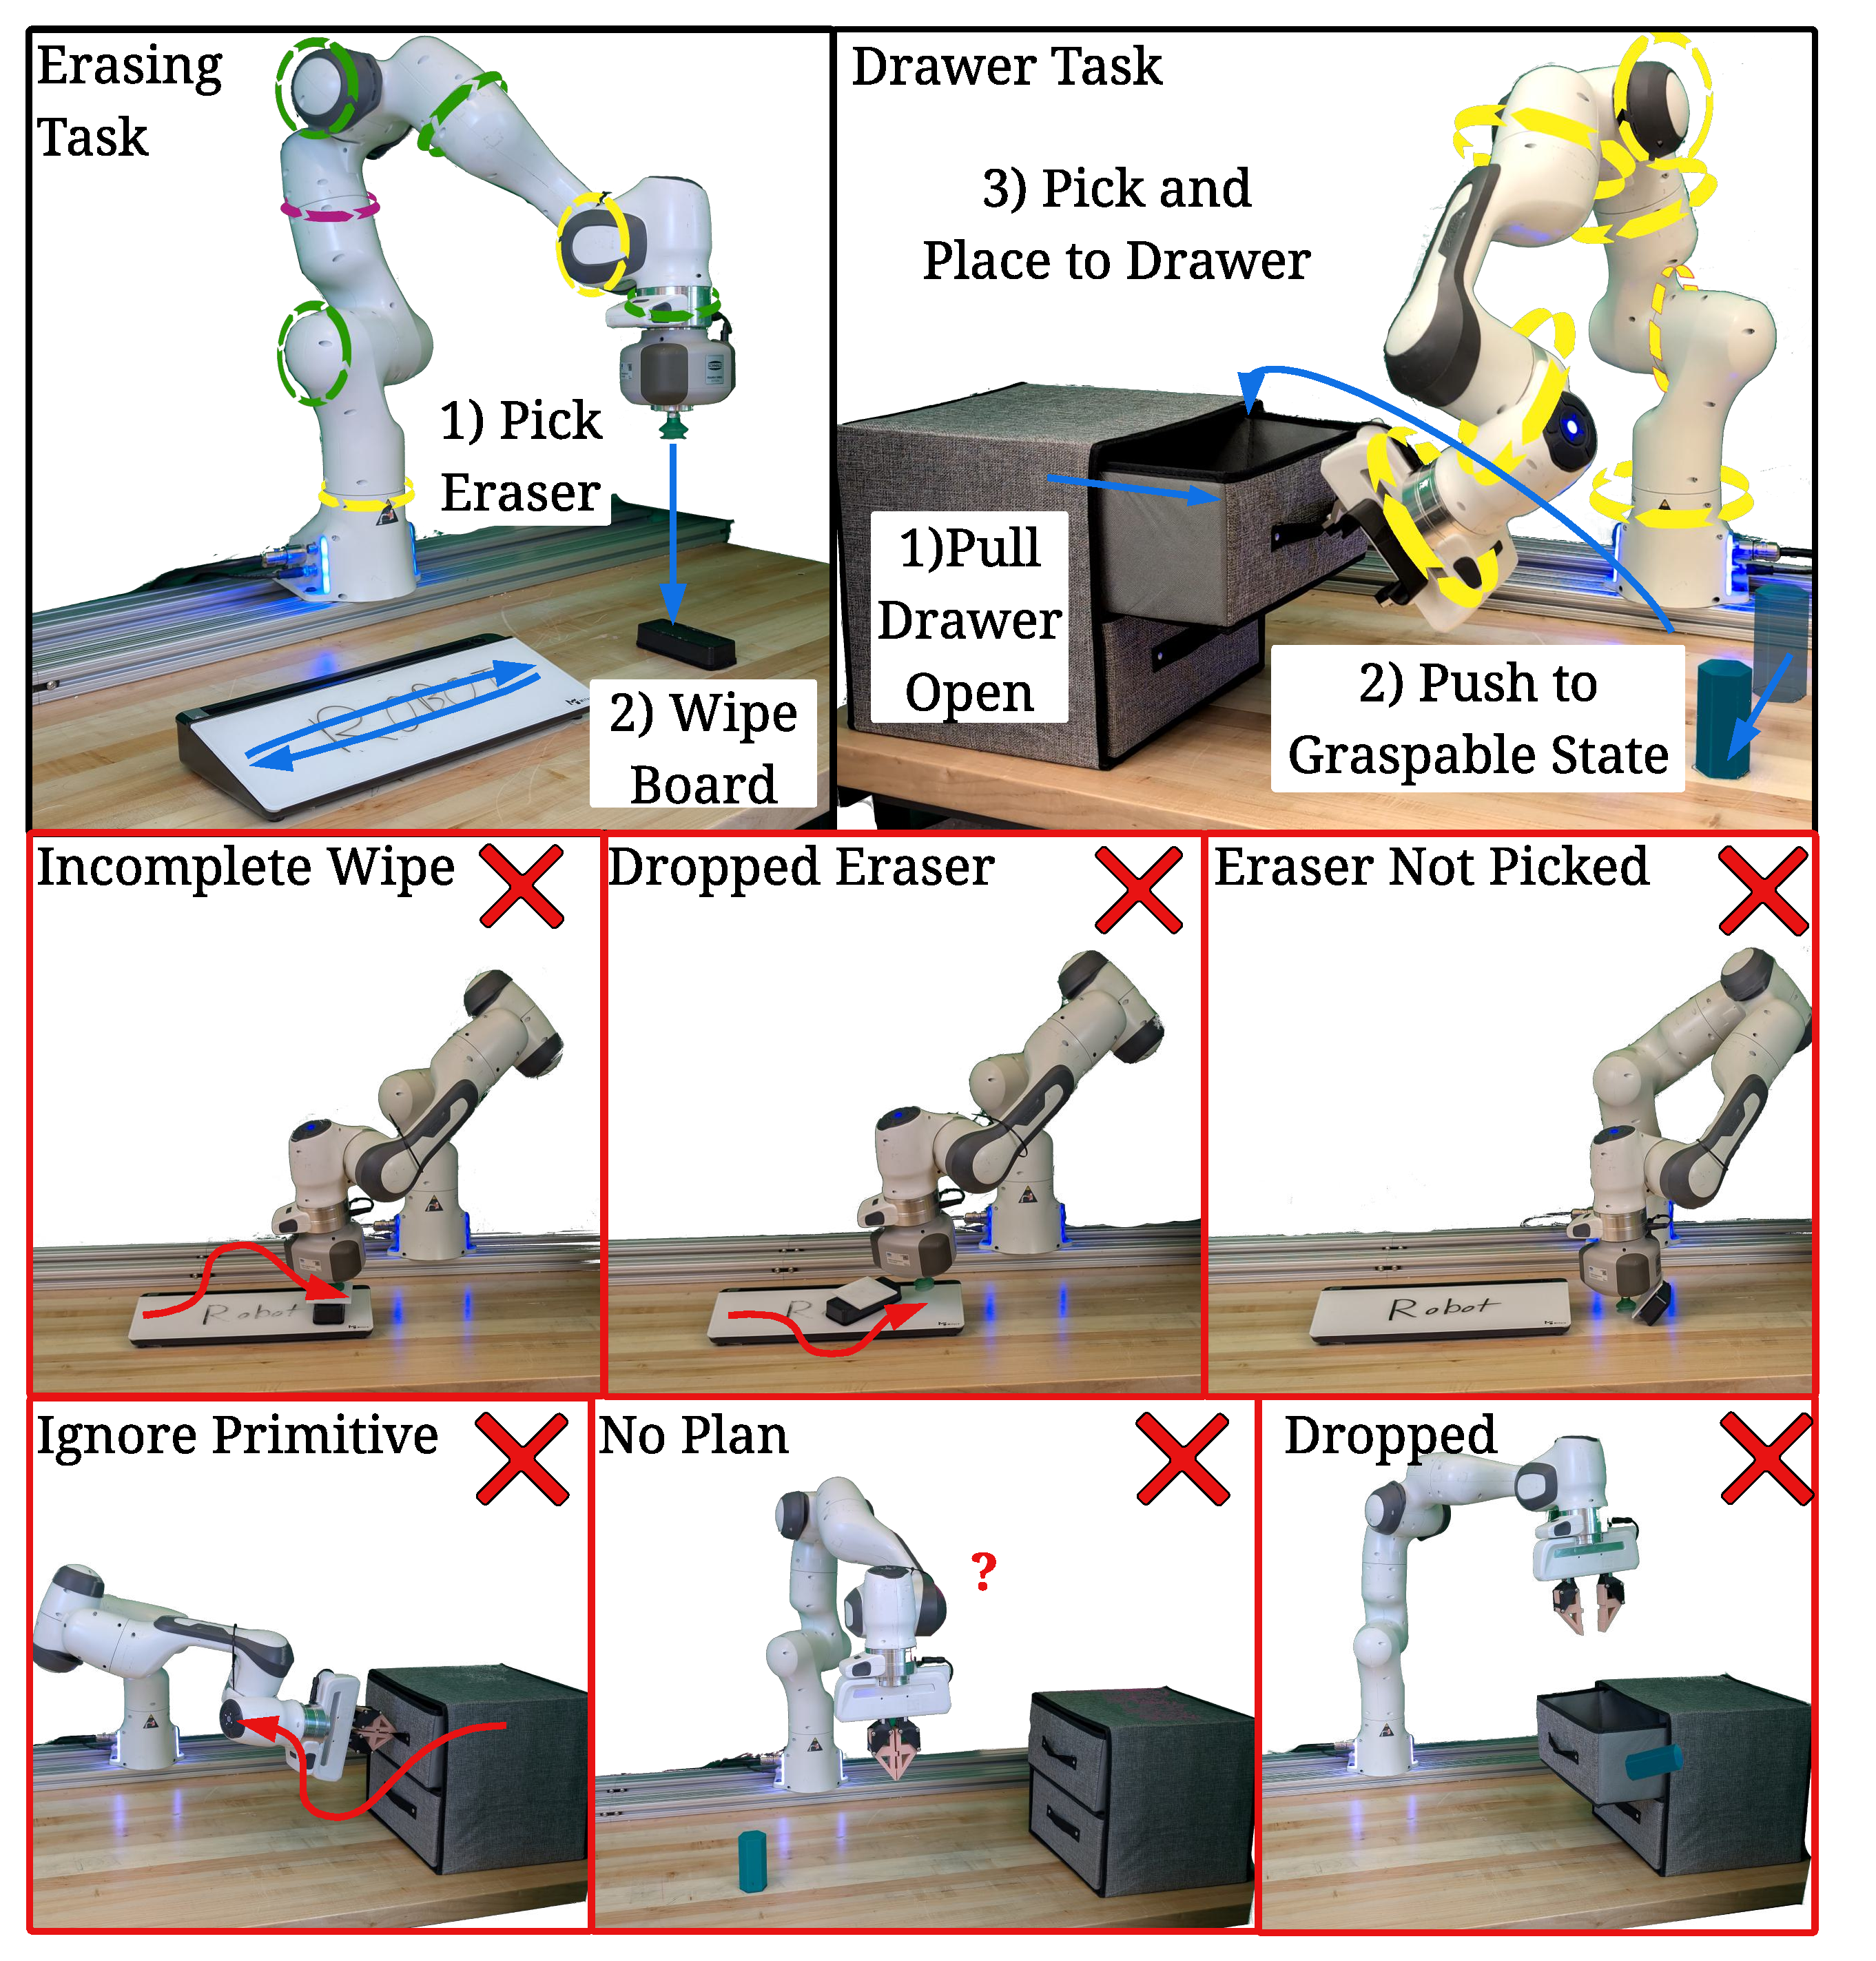
\includegraphics[width=\columnwidth]{../movingon/figures/real-task-explainer-vertical-compressed-1.pdf}
  \caption{Left (Erasing): The robot grasps an eraser from the table and performs back-and-forth sweeps to remove text. Right (Drawer): The robot opens a drawer, pushes an object to a graspable pose, places it inside, and closes the drawer.}
  \label{fig:deft:real}
\end{figure}

We test DEFT on two long-horizon, multi-primitive tasks (\cref{fig:deft:real}). The \textit{Drawer Task} consists of five sequential phases: pulling the drawer open, pushing the object to a graspable position, grasping, placing the object inside, and pushing the drawer closed. The \textit{Erasing Task} requires grasping an eraser from the table and sweeping it back and forth across a whiteboard to remove pre-written text. Together these tasks demand transitions between unconstrained free-space motion and constrained contact-rich interaction.

\begin{table}[h]
\centering
\caption{Real-world task results over 10 runs.}
\label{tab:deft:rw}
\begingroup
\setlength{\tabcolsep}{5pt}
\renewcommand{\arraystretch}{1.1}
\footnotesize
\begin{tabular}{@{}llcc@{}}
\hline
\textbf{Model} & \textbf{Task} & \textbf{Mean} & \textbf{Std.}  \\
\hline
DEFT                & Drawer  & \textbf{1.00} & 0.00  \\
DEFT                & Erasing & \textbf{1.00} & 0.00 \\
Optimization        & Drawer  & 0.00 & 0.00 \\
Optimization        & Erasing & 0.35 & 0.32 \\
DEFT-NoConditioning & Drawer  & 0.60 & 0.49 \\
DEFT-NoConditioning & Erasing & 0.93 & 0.12 \\
\hline
\end{tabular}
\endgroup
\end{table}

\textsc{DEFT} achieved perfect task completion on both real-world tasks (\cref{tab:deft:rw}). The Optimization baseline produced no executable plans on the drawer task. \textsc{DEFT}-NoConditioning succeeded in 6/10 drawer runs and 9.3/10 erasing runs, with failures attributable to missing embodiment conditioning and inpainting causing surface-constraint violations. These outcomes support our central hypothesis: embodiment and task conditioning, coupled with inpainting and clamping, yield a policy that remains fail-active under embodiment degradation.

Comparing against the sampling-based approach from Chapter~\ref{ch:constrained}, DEFT removes the need for pre-computation of kinodynamic action maps and generalizes to previously unseen failure conditions at inference time---directly addressing the computational demand limitation identified in that work. The cost is the loss of formal completeness guarantees, which sampling-based kinodynamic methods provide under certain conditions.
